\documentclass[11pt]{article}
\usepackage[UTF8,heading=false,fontset=fandol]{ctex}
\usepackage{fontspec}
\IfFontExistsTF{TeX Gyre Termes}{\setmainfont{TeX Gyre Termes}}{\IfFontExistsTF{Times New Roman}{\setmainfont{Times New Roman}}{\setmainfont{lmroman10}[Extension=.otf,UprightFont=*-regular,BoldFont=*-bold,ItalicFont=*-italic,BoldItalicFont=*-bolditalic]}}
\IfFontExistsTF{TeX Gyre Heros}{\setsansfont{TeX Gyre Heros}}{\setsansfont{lmsans10}[Extension=.otf,UprightFont=*-regular,BoldFont=*-bold,ItalicFont=*-oblique,BoldItalicFont=*-boldoblique]}
\usepackage[numbers,sort&compress]{natbib}
\usepackage{microtype}
\usepackage{booktabs}
\usepackage{graphicx}
\usepackage{tabularx}
\usepackage{float}
\usepackage{hyperref}
\usepackage{memmy-review}
\hypersetup{colorlinks=true,linkcolor=MemmyAccent,citecolor=MemmyAccent,urlcolor=MemmyAccent}
\renewcommand{\memmyreviewlabel}{文献综述}
\renewcommand{\memmyabstractlabel}{摘要}
\renewcommand{\memmygeneratedby}{由 Memmy 文献综述插件生成}
\renewcommand{\memmydisclaimer}{AI 生成，仅供参考，不支持正式投稿。}
\renewcommand{\memmyfullnotice}{本综述由 AI 生成，仅供参考，不支持用于正式学术投稿。使用者应自行核验全部事实、引文和参考文献。}
\renewcommand{\refname}{参考文献}
\title{智能体长期记忆：从证据到知识的持续演化}
\begin{document}
\maketitle

\begin{abstract}
本文以智能体长期记忆为主题，展示 Memmy 文献综述的品牌排版。围绕来源管理、证据组织、检索综合与版本修订，样例呈现完整的标题层级、正文段落、流程图、比较表及引用。本文内容为版式演示，图表和参考条目不构成真实研究证据。
\end{abstract}

\section{从信息积累到可追溯记忆}

长期记忆的目标，是把分散的交互与文献信息组织为能够持续检索、核验和修订的知识。对于文献综述而言，保存一段流畅的总结只是起点：更关键的是知道总结来自何处、适用于什么条件，以及新证据出现后应该如何更新。

一个清晰的记忆流程，可以从来源导入、证据索引、检索综合和审计更新四个阶段展开。各阶段保留相互关联的记录，使读者能够从正文中的论断回到原始材料。本页的流程图仅用于展示版式，不表示实验结论。

\begin{figure}[H]
\centering
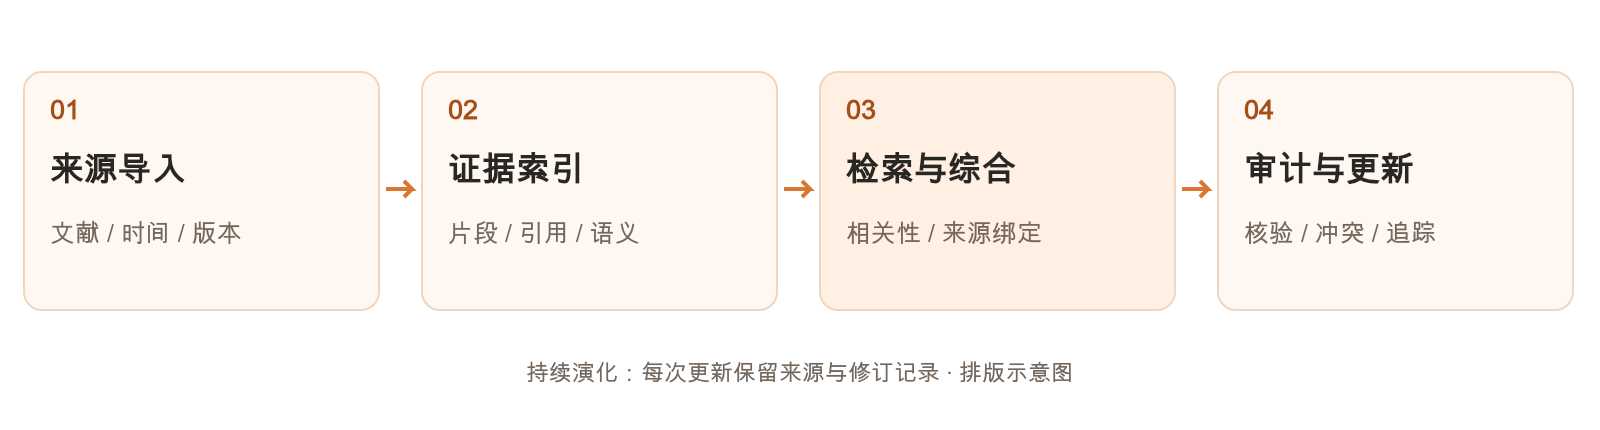
\includegraphics[width=0.92\linewidth,height=0.45\textheight,keepaspectratio]{assets/figures/lifecycle-source.png}
\caption{从来源到修订的记忆工作流。图中流程为版式示意，非实验结果。}
\label{fig:lifecycle-block}
\end{figure}

\section{记忆系统的设计取舍}

系统设计需要兼顾检索质量、更新成本和可解释性。直接保存原始片段便于核查，结构化关系有助于组织跨文献联系，压缩后的摘要则便于快速浏览。这些表示可以组合使用，具体取舍应围绕任务需求与证据条件展开。

\subsection{检索与证据绑定}

检索结果应同时保留内容与出处，并向写作阶段传递明确的证据边界。生成时应区分直接观察、跨文献综合与尚待验证的判断，避免把相近的语义误认为相同的结论。多来源的一致性也需要结合时间、对象和实验条件理解。

\subsection{冲突处理与版本管理}

当新旧材料存在差异时，保留修订关系比直接覆盖旧结论更有价值。版本记录应说明新增证据、受影响的论断以及更新原因。这样既便于恢复历史状态，也使后续审计能够准确定位变化。

\section{评估与开放问题}

评估不应仅关注是否检索到一段相关文字，还应检查来源是否完整、论断能否核验、更新是否保留历史，以及引用是否与正文一致。下表以示意性条目展示三种常见的组织思路，所有描述仅用于排版预览。

开放问题集中在长期维护与跨任务复用：系统如何识别过时信息，如何在成本可控的条件下保留证据多样性，以及如何向使用者清楚呈现结论的适用范围。实际综述应针对明确的研究问题，以经过核验的材料替换这些演示段落 \cite{LayoutDemo2026}。

\begin{table}[H]
\centering
\small
\caption{记忆组织方式的示意比较（排版演示）。}
\label{tab:comparison-block}
\begin{tabularx}{\linewidth}{>{\hsize=0.633\hsize\linewidth=\hsize\raggedright\arraybackslash}X >{\hsize=1.267\hsize\linewidth=\hsize\raggedright\arraybackslash}X >{\hsize=1.100\hsize\linewidth=\hsize\raggedright\arraybackslash}X}
\toprule
\rowcolor{MemmyTint} \textbf{组织方式} & \textbf{主要用途} & \textbf{维护重点} \\
\midrule
原始片段 & 保留上下文，支持回溯核验 & 来源与版本标识 \\
结构化关系 & 连接对象、方法与跨文献观点 & 关系更新与冲突记录 \\
摘要与索引 & 概览主题，辅助检索定位 & 过时检测与证据绑定 \\
\bottomrule
\end{tabularx}
\end{table}

\begin{thebibliography}{99}
\small
\raggedright
\setlength{\itemsep}{0.18em}
\setlength{\parsep}{0pt}
\bibitem{LayoutDemo2026} Memmy. (2026). 排版演示条目（非真实文献）
\end{thebibliography}
\end{document}
